% Ashwin Madavan
\documentclass{article}
\usepackage{graphicx, subfig, amssymb, wrapfig, lipsum, hyperref, movie15}
\graphicspath{{./img/}}
\hypersetup{
    colorlinks=true,
    linkcolor=blue,
    filecolor=magenta,      
    urlcolor=cyan,
}
\begin{document}

\title{Project 3: PacMan}
\date{April 2, 2015}
\author{Ashwin Madavan}
\maketitle

\section{Introduction}
\begin{wrapfigure}{r}{0.5\textwidth}
	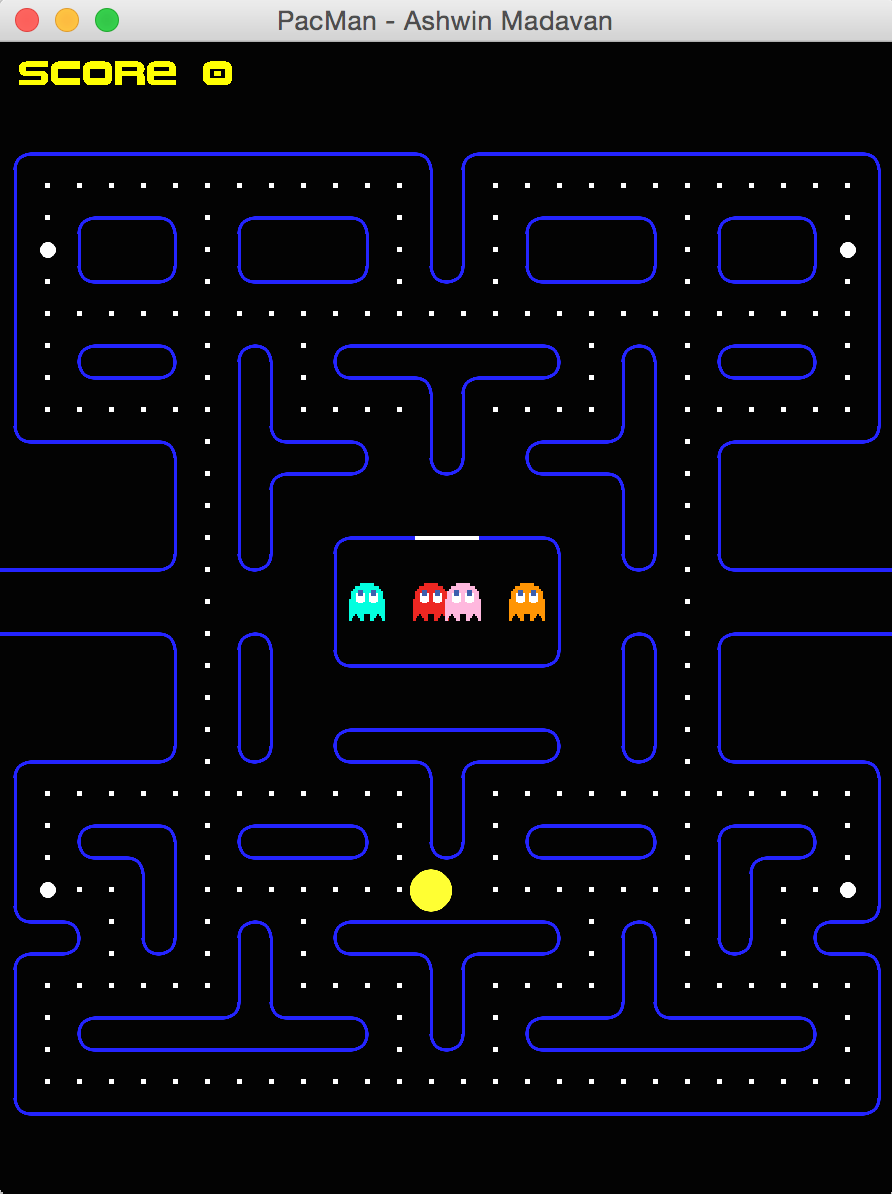
\includegraphics[width=0.48\textwidth]{game}
	\caption{Game Screenshot \label{f:screenshot}}
\end{wrapfigure}

PacMan was designed by Toru Iwatani in 1980, and quickly became a popular arcade
game. I re-created Pacman in Java and desgined and trained a neural net to play
the game for me. While everything that you see will see below including images,
code, and words are all mine, I did receive a lot of information regarding the
mechanics of the game from the
\href{http://home.comcast.net/~jpittman2/pacman/pacmandossier.html}{Pacman
Dossier}. I encourage you to \href{http://www.playpacmanonline.net/}{play} the
original game online before reading through the rest of this report.

\subsection{Playing PacMan}
The code base was designed with extensibility and generality in mind. To run the
game, simply run pacman.jar. The parameters of the game can be tweaked by
adjusting the pacman.properties file. A description of each property is included
in the properties file.

\subsection{Mechanics}
While the basic gameplay of PacMan is common knowledge, the inner mechanics of
the game are much less well known. The sections below will attempt to explain
some of the more interesting components of the game.

\subsubsection{Ghosts}
\begin{figure}[h]
	\centering
	
\includegraphics[width=0.75\linewidth]{actors}
	\caption{Pinky, Inky, Clyde, Blinky, and PacMan \label{f:actors}}
\end{figure}

There are four ghosts in PacMan: Blinky, Clyde, Inky, and Pinky. Ghosts exist in
one of three modes: chase, scatter, frightened, and eaten. When the ghosts are
in the chase or scatter modes, they move by attempting to reach a target tile in
the grid. Whenever a ghost reaches an intersection, it turns in the direction
that will minimize its distance to its target location. This target tile is a
fixed location in the corners of the map during scatter mode and is a variable
location relative to PacMan and the other ghosts' positions during chase mode.
In frightened mode, ghosts randomly select a direction to turn in whenever they
reach an intersection. In the eaten mode, consumed ghosts return back to their
initial position to respawn.

During chase mode, each ghost has a different targeting scheme. Blinky targets
PacMan's current position. Pinky targets the tile four in front of PacMan's
current position. Inky targets the position formed by doubling the vector from
Blinky to the position two in front of PacMan. Clyde's target changes depending
on his proximity to PacMan. If he is within eight tiles, Clyde's target is the
same as his scatter target. Otherwise, his target is exactly the same as Blinky.

\subsubsection{Scoring}
PacMan earns points by eating food and energizers and by consuming ghosts.
PacMan earns 10 points for food, 50 points for energizers, and $200 *
2^{ghosts}$ points for ghosts.

\section{Discussion}
\subsection{Solution Design}
The sections below attempt to explain some of the most important aspects of
my solution design. For a more complete picture of how the code behaves, please
refer the the javadocs (/docs/javadoc) and to the code itself.

\subsubsection{Grid}
\begin{figure}[h]
	\centering
	
\includegraphics[width=0.75\linewidth]{terrain}
	\caption{Empty, Food, Energizer, Walls, and Gate \label{f:terrain}}
\end{figure}

There are ten different types of terrain that are arranged in a two-dimensional
grid to form the playing field. Some terrain is passable (e.g., empty and food),
others are impassable (e.g., walls), and others still are passable under certain
circumstances (e.g., gates when ghosts are eaten).

New maps can be also be added and played. Maps consist of two files: a text file
(.txt) and a properties file (.properties). The text file consists of the
numbers and characters. The numbers correspond to the ordinals of the terrain
(e.g, empty -> 0, horizontal wall -> 3, etc.). Upper case B, C, I, P, and M
specify the starting position of Blinky, Clyde, Inky, Pinky, and Pacman
respectively. Lower case b, c, i, and p specify the target for Blinky, Clyde,
Inky, and Pinky in scatter mode. Upper case E specifies the exit of the ghost
house (where ghosts begin each round).

\subsubsection{Actors}
The Actor class represents the highest level of abstraction of agents in the
game. Actors are movable and orientable. The current position of an actor is the
pixel coordinates of its center point. While actors move independently of the
grid, their position is translated into a tile for the purposes of collision
detection. Actors occupying the same tile are said to have collided.

Actors also have an orientation. All orientation shifts must happen when the
actors are in a center of a tile. This prevents actors from moving off the grid
lines while still enabling them to move at arbitrary speeds.

\subsubsection{Sprites}
All of the images displayed in the game are my custom creation. They were
designed in GIMP 2.8. The original .xcf files are included in the assets/sprites
folder to prove that they were my creations.

The sprites are organized in a sprite sheet. By placing all images into a single
file, I significantly reduce the number of image files that the program needs to
load and keep track of during execution. Sprites are represented in the program
as indicies within the sprite sheet. These indicies are translated into absolute
coordinates when the sprite is drawn.

\subsubsection{Game}
The Game class manages all the various entities within the program. It contains
the logic that moves actors within the grid and that detects win and loss
conditions. By itself, the Game class is headless. The GraphicalGame class
adds graphical functionality to the headless game.

\subsection{Artificial Intelligence}
I designed a neural net and evolved it using a genetic algorithm to develop a
smart ai to play PacMan. The core genetic algorithm code is essentially
identical to the code that I submited for lab 1. Because the code was so
extensible, all I had to do was add a custom fitness calculator to get the
algorithm to run!

\subsubsection{Neural Net}
I designed my neural net to be highly generalized so that I can include it in
future projects. My neural net is a feed-forward network that utilizes a sigmoid
function to output non-binary results. The network itself can be serialized to
files so that trained networks can be saved for future use.

My network for PacMan has two hidden layers comprised of ten and eight neurons
respectively. There are twelve inputs to the neural network, which are (1) the
distance from the ghosts to PacMan, (2) whether or not the ghosts are moving
toward PacMan, (3) the mode that the ghosts are in, (4) the location of the
closest food, and (5) the location of the closest energizer. The outputs of the
neural network are four values in the range $[0, 1]$. Each output corresponds to
a different orientation. PacMan selects the valid orientation with the highest
output to determine which direction to turn to.

\subsubsection{Training}
Fitness was determined by $1 / (e + s(W))$, where $s(W)$ is the score from the
game where the weights of the neural network are W and e is the elapsed time.
This is because we want to find the network that produces behavior that allows
the PacMan to stay alive the longest and to produce the most points. We take the
inverse, because the genetic algorithm is designed to minimize fitness.

\subsubsection{Performance}
The neural network was evolved for 25 generations using a genetic algorithm.
The result survived for 22 seconds and earned 1740 points! For a full video of
the network playing pacman, please refer to /docs/pacman-ai.mov.

In comparison, a randomly generated neural network earned an average of 86.4
points over five trials. Clearly, the training process significantly improved
the network weights.

\end{document}